% !TeX root = ../tfg.tex
% !TeX encoding = utf8

\chapter{Experimentación}
\label{cap:capitulo4}

A lo largo del presente capítulo se expondrán los resultados obtenidos tras la aplicación de varios algoritmos relacionados con ataques adversario, culminando con un ataque diseñado por el propio estudiante teniendo en cuenta los conceptos aprendidos a lo largo de la carrera. Todos ellos se centrarán en redes neuronales convolucionales, en específico en una red: el objetivo de esta red neuronal basada en LeNet es la detección de señales alemanas en conducción autónoma. La red ya ha sido entrenada y el modelo ha sido descargado del repositorio GitHub del autor, y su implementación se ha realizado usando Keras, Tensorflow y Numpy.

Se han implementado tres algoritmos que simulan ataques exploratorios en el mundo real, siendo uno de ellos propuesto por el estudiante basado en algoritmos de optimización. Además, se usan varios parámetros para comprobar el funcionamiento del algoritmo en cada señal. Finalmente, se llegará a la conclusión de que, si se busca la no detección del ataque, no será válido aplicar un algoritmo a cualquier imagen.

Las implementaciones se han realizado en un Notebook, en el entorno de Google Colab (puede encontrarse en Rodríguez-Gallardo et al.~\cite{MiGithub}. Además, los ataques se centrarán en torno a las imágenes que aparecen en la figura Fig~\ref{fig:senales_limpias}.


\begin{figure}[h]
    \centering
        \centering
        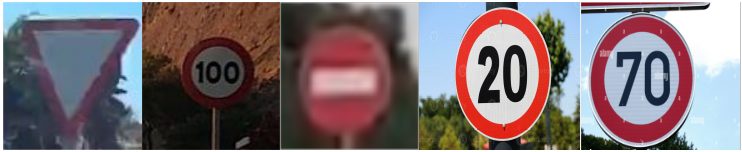
\includegraphics[width=\textwidth]{img/todas_senales_limpias.png}
        \caption{Imágenes usadas en los ataques. De izquierda a derecha: ceda el paso, máximo a $100$ km/h, dirección prohibida, máximo a $20$ km/h y máximo a $70$ km/h}
        \label{fig:senales_limpias}
\end{figure}

\section{Ataque teórico}

El primer ataque presentado tiene como objetivo demostrar que lo buscado en los desarrollos teóricos tiene sentido. Esto es, siempre se cumple lo siguiente: para toda imagen $x \in \mathbb{R^{n \times m}}$, existe un $\delta \in \mathbb{R^{n \times m}}$ de tal manera que si $f$ clasifica $x$ correctamente, entonces $f(x + \delta) \neq f(x)$.

Nótese que estos experimentos sirven para demostrar que todos los datos tienen asociada, al menos, una modificación de tal manera que hace que el modelo falla. En la realidad, los objetivos del atacante puede ir más allá de simplemente hacer que el modelo falle: el modelo debe clasificar $x+\delta$ como una clase en específico o los datos alterados no deben ser detectados, entre otros requisitos.

Para la construcción de $\delta$, se opta por suponer normalidad en la distribución del ruido, teniendo en cuenta que como no se busca que se detecte el ruido, la normal tiene vector de medias nulo (ya que este valor indica que el ruido debe obtenerse tomando como referencia el valor del píxel de la imagen original, según la varianza considerada por píxel). Respecto a la matriz de convarianzas, se consigue una implementación donde a partir de la varianza por píxel se consigue obtener $\delta$ sin el uso de la mencionada matriz.

Los resultados aparecen en las imágenes que aparecen en las figuras Fig~\ref{fig:cedapasoteorico}
, Fig~\ref{fig:max100teorico}, Fig~\ref{fig:dir_prob_teorico}, Fig~\ref{fig:max70teorico} y Fig~\ref{fig:max20teorico}.


\begin{figure}[H]
    \centering
        \centering
        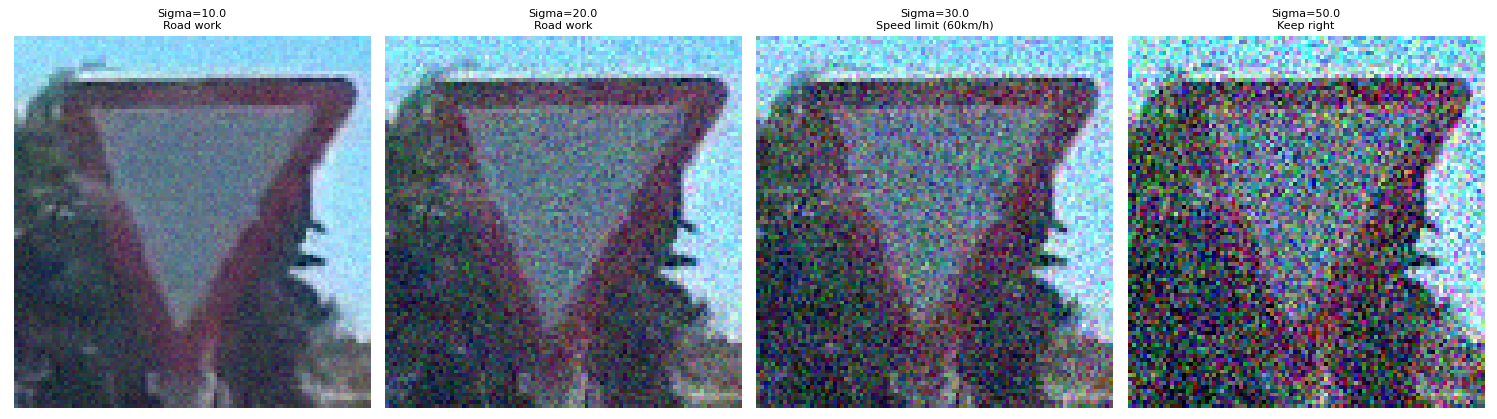
\includegraphics[width=\textwidth]{img/cedaPasoTeorico.png}
        \caption{Ataque teórico a la imagen de ceda el paso con su respectiva predicción}
        \label{fig:cedapasoteorico}
\end{figure}

\begin{figure}[H]
    \centering
        \centering
        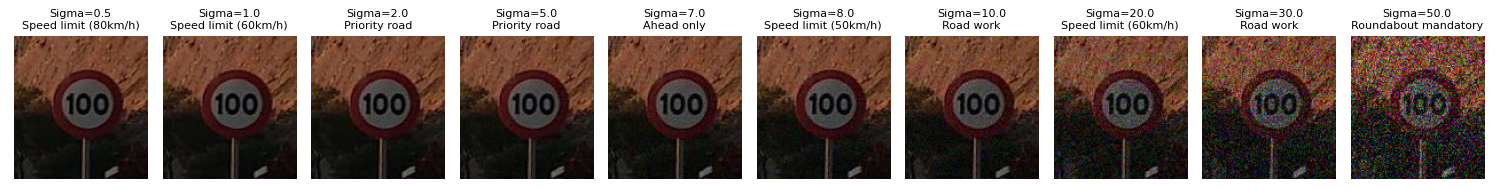
\includegraphics[width=\textwidth]{img/max_100_teorico.png}
        \caption{Ataque teórico a la imagen de máximo a $100$ km/h con su respectiva predicción}
        \label{fig:max100teorico}
\end{figure}

\begin{figure}[H]
    \centering
        \centering
        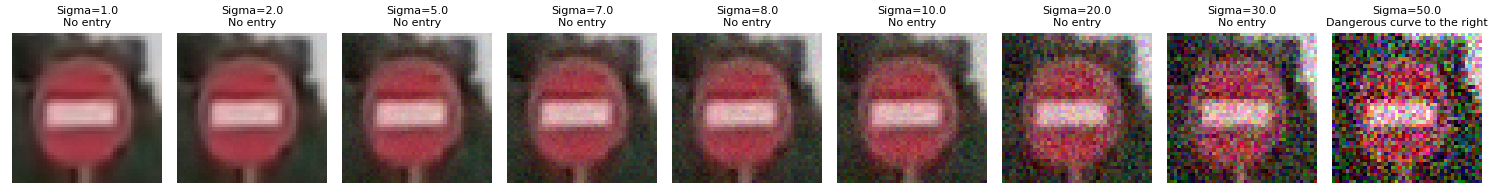
\includegraphics[width=\textwidth]{img/dir_prohib_teorico.png}
        \caption{Ataque teórico a la imagen de dirección prohibida con su respectiva predicción}
        \label{fig:dir_prob_teorico}
\end{figure}

\begin{figure}[H]
    \centering
        \centering
        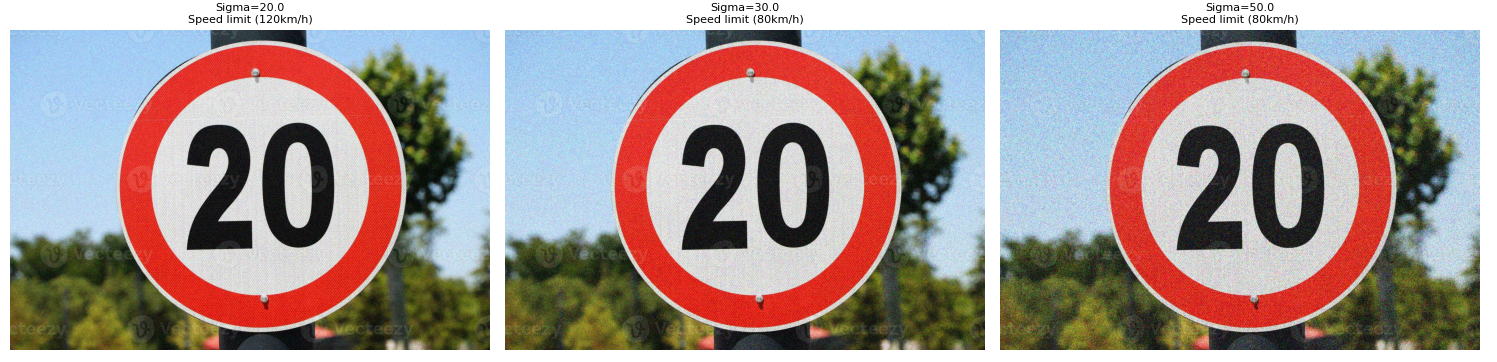
\includegraphics[width=\textwidth]{img/max_20_teorico.png}
        \caption{Ataque teórico a la imagen de máximo a $20$ km/h con su respectiva predicción}
        \label{fig:max20teorico}
\end{figure}

\begin{figure}[H]
    \centering
        \centering
        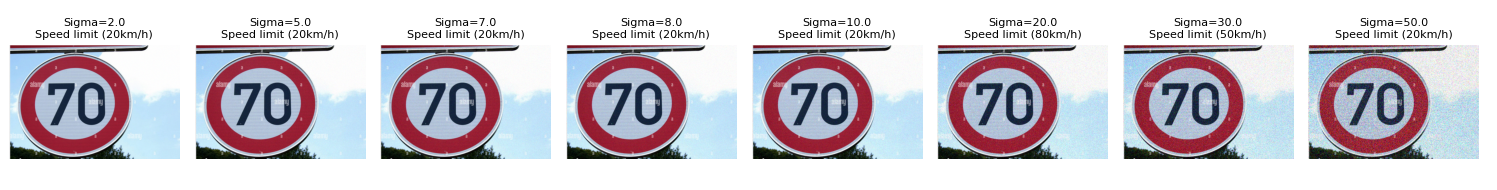
\includegraphics[width=\textwidth]{img/max_70_teorico.png}
        \caption{Ataque teórico a la imagen de máximo a $70$ km/h con su respectiva predicción}
        \label{fig:max70teorico}
\end{figure}

Nótese que el mínimo valor de la desviación típica (en consecuencia, de la varianza) para el que la imagen comienza a ser mal clasificada es distinto según las características de cada una y, presumiblemente, de las propiedades del modelo empleado. En la imagen que aparece en la figura resumen Fig~\ref{fig:tablaresumenteorico} se puede observar más fácilmente la diferencia por imagen según la desviación típica escogida.

Con esto se consigue ver experimentalmente que el objetivo buscado por los desarrollos teóricos es cierto. Sin emaargo, tal y como se comentó, carecen de interés si se busca que, dada la imagen, el modelo la clasifique de determinada forma.

\begin{figure}[H]
    \centering
        \centering
        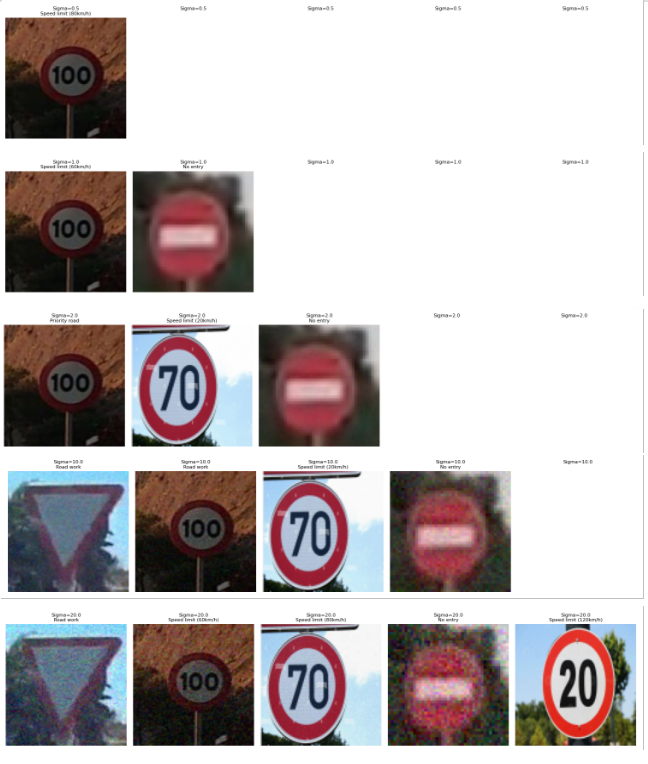
\includegraphics[width=\textwidth, height=\textwidth]{img/tabla_resumen_teorico.png}
        \caption{Resumen de las distintas situaciones de ataque teórico. Cada fila corresponde a un valor de desviación típica, y solo aparecen las imágenes para las que el clasificador ha sido engañado. Desviación típica de arriba abajo: $0.5$,$1.0$,$2.0$,$10.0$,$20.0$}
        \label{fig:tablaresumenteorico}
\end{figure}

\section{FGSM}

Uno de los ataques más conocidos en el ámbito de los ataques exploratorios es el ataque \textit{Fast Gradient Signed Method}, o FGSM. El objetivo es el de obtener cierto $\epsilon \in [0,1]$ para el que el modelo falla la predicción cuando se altera la imagen según la expresión expuesta en el capítulo anterior. A continuación, en la imagen que aparece en la figura Fig.~\ref{fig:tablaresumentfgsm}, aparece un resumen de los resultados experimentales obtenidos tras aplicar FGSM para varios valores de $\epsilon$, probando en un principio con un valor muy pequeño, hasta valores más grandes. Obsérvese que a mayor valor de $\epsilon$, más fácil es detectar la imagen alterada, por lo que aunque es un método fácil de implementar y no es necesario conocer más información de la red más allá del gradiente, no sería el más recomendado de los existentes en la literatura.

\begin{figure}[H]
    \centering
        \centering
        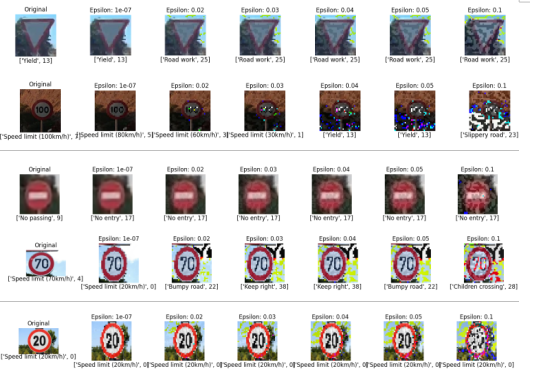
\includegraphics[width=\textwidth]{img/tabla_resumen_fgsm.png}
        \caption{Resumen de las distintas situaciones de ataque FGSM. Por columna, la ataque original, $\epsilon=10^{7}$,$\epsilon=0.02$,$\epsilon=0.03$,$\epsilon=0.04$,$\epsilon=0.05$ y $\epsilon=0.1$}
        \label{fig:tablaresumentfgsm}
\end{figure}

Nótese que, al igual que en los ataques teóricos, es necesario estudiar el valor de $\epsilon$ adecuado para hacer que el clasificador falle

\section{Optimización con búsqueda local}

El presente algoritmo de ataque se basa en el expuesto en el capítulo anterior, el cual era un ataque no etiquetado, con la diferencia de que tras una serie de ajustes, se ha transformado en un ataque etiquetado. Este tipo de ataques son bastante más interesantes que los no etiquetados, tal y como se verá a continuación.

Se presentan dos situaciones de ataque en el mundo real:

\begin{itemize}
    \item Un vehículo autónomo circula en una vía donde la máxima velocidad permitida es de $70$ km/h (y como normalmente se encuentran fuera de autovías o autopistas, la velocidad mínima corresponde a $35$ km/h).

    \item De nuevo un vehículo controlado por una inteligencia artifical detecta una señal de dirección prohibida, por lo que debe parar o circular por otro lugar donde la señal no sea válida.
\end{itemize}

Basado en algoritmos para optimización, el alumno propone el uso de búsqueda local intentando maximizar la probabilidad de salida de que cierta imagen sea etiquetada como desea el atacante. En este caso, la etiqueta con la que se busca clasificar es la asociada a la imagen de señal de máximo a $20$ km/h. De esta manera, el ataque es además de caja negra, siendo necesario únicamente realizar predicciones en la red víctima.

Se ha seguido el esquema de "mejorar cuando se encuentre una solución que mejore la actual". Para generar los vecinos, se escoge una posición aleatoria en la solución actual y se añade ruido gaussiano en un entorno cuadrado de dicho píxel, con dimensiones prefijadas. La solución entonces se actualizará cuando mejore el valor de la función objetivo. Es decir, aumenta la probabilidad de que la red clasifique la imagen como quiere el atacante (en este experimento, etiqueta de máxima velocidad a $20$ km/h).

En el primer caso, la señal de máxima velocidad a $70$ km/h es introducida como solución inicial en búsqueda local. El algoritmo entonces devuelve la imagen que aparece en la figura Fig~\ref{fig:blmax70}. Puede observarse que la diferencia con la imagen limpia es prácticamente nula, por lo que cumple el requisito de ser difícilmente reconocible, y la probabilidad de que la señal sea máxima velocidad $20$ km/h es prácticamente $1$.

\begin{figure}[H]
    \centering
        \centering
        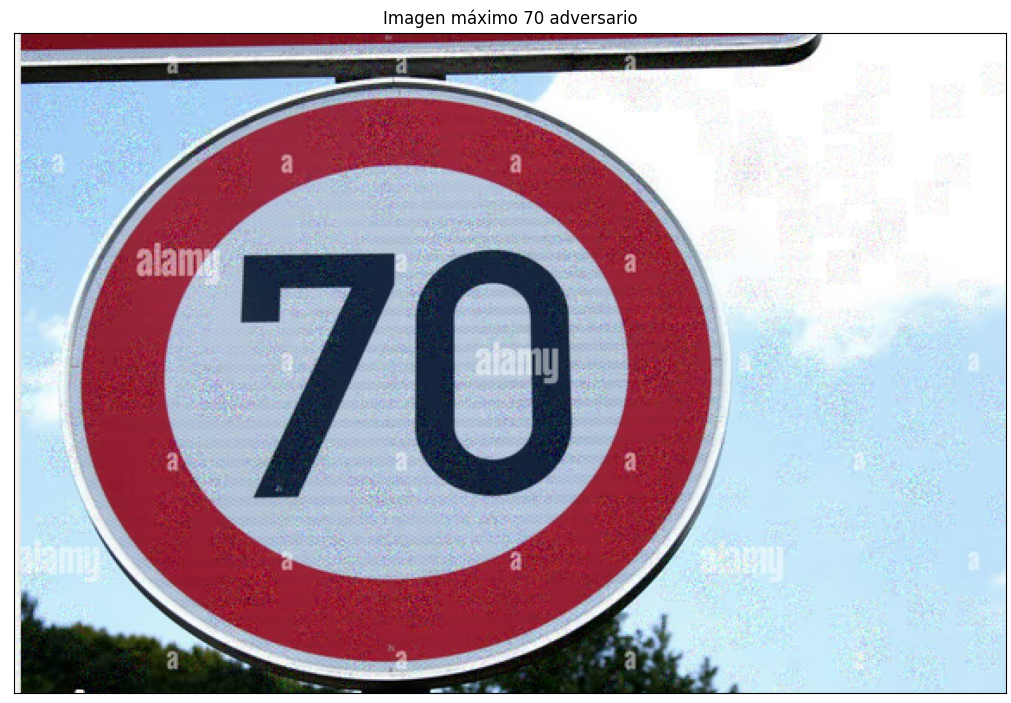
\includegraphics[width=\textwidth]{img/max_70_detectada_como_max_20.png}
        \caption{Señal de máximo $70$ km/h alterada con búsqueda local}
        \label{fig:blmax70}
\end{figure}

Es conveniente estudiar la convergencia del método. En la imagen que aparece en la figura Fig~\ref{fig:evolucion1}. La probabilidad inicial de que la imagen sea clasificada como máximo a $20$ km/h es cercana a $0.3$, y antes de la iteración $150$ el algoritmo ha conseguido obtener una solución cuya probabilidad de que el modelo clasifique según se ha especificado está entre $0.9$ y $1.0$. Teniendo en cuenta que el número máximo de iteraciones es de $1000$, la probabilidad de que clasifique como se quería es casi $1$ y ha convergido rápido a una imagen que apenas parece haber sido modificada, se puede concluir que el ataque ha sido exitoso.

\begin{figure}[H]
    \centering
        \centering
        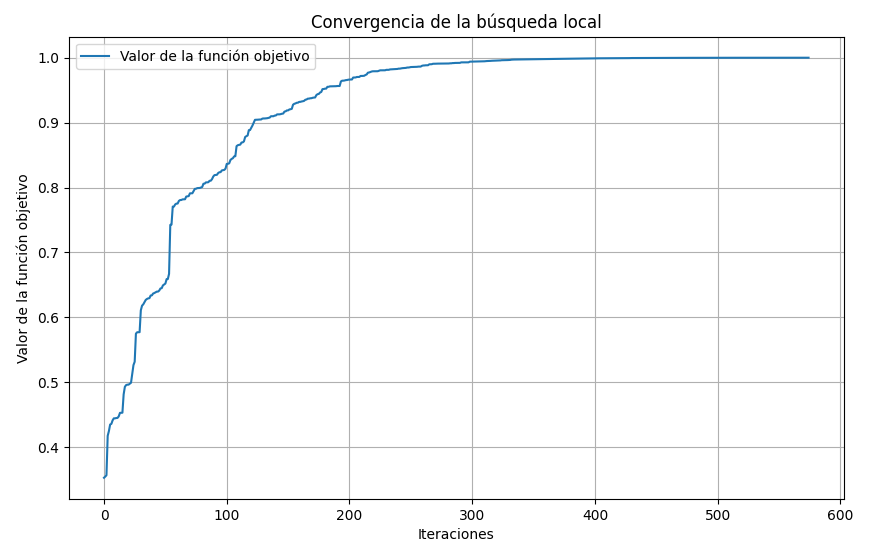
\includegraphics[width=\textwidth]{img/evolucion_max_70_bl.png}
        \caption{Convergencia de búsqueda local para la señal de máximo a $70$ km/h}
        \label{fig:evolucion1}
\end{figure}

Respecto al segundo caso, la imagen obtenida al final del algoritmo aparece en la figura Fig~\ref{fig:dirprohibbl}. Es muy fácil darse cuenta en este caso que la imagen ha sido alterada, y se pueden tomar medidas para evitar un posible accidente. Si bien es cierto que obviando la detección de la muestra, la probabilidad de que la red clasifique la imagen como máximo $20$ km/h es $1.0$, por lo que el objetivo del diseño del algoritmo ha sido conseguido.

\begin{figure}[H]
    \centering
        \centering
        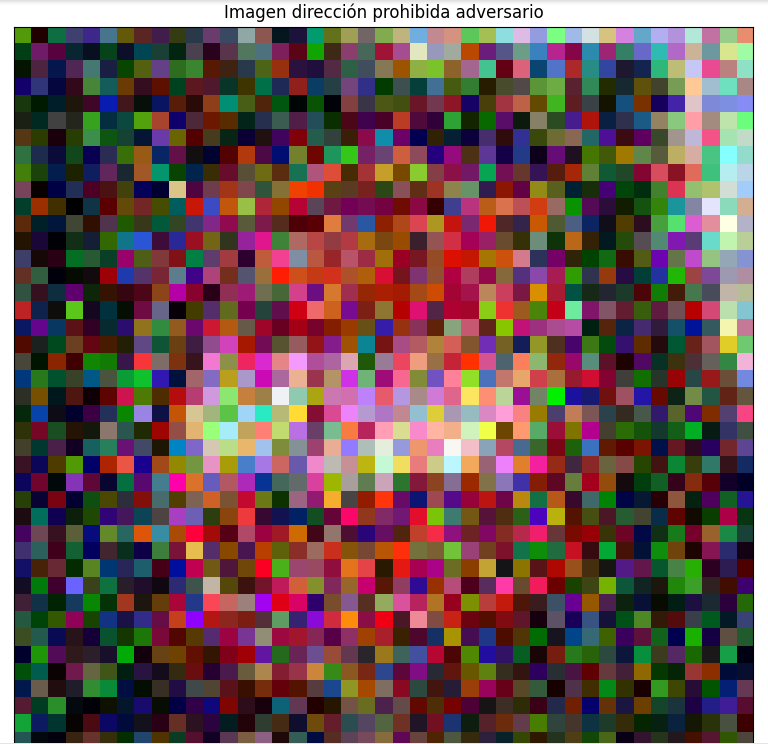
\includegraphics[width=0.5\textwidth,height=0.5\textwidth]{img/dir_prohib_detectada_como_max_20.png}
        \caption{Señal de dirección prohibida alterada con búsqueda local}
        \label{fig:dirprohibbl}
\end{figure}

También se estudia la convergencia del método en este caso. La gráfica puede observarse en la figura Fig~\ref{fig:evol2}. A diferencia de la curva de convergencia del primer caso, que tenía un crecimiento suave, la curva de la señal de dirección prohibida empieza en una probabilidad de clasificación de $0.0$, con un comienzo bastante lento. En pocas iteraciones, la curva tiene un crecimiento casi exponencial, siendo este más acrecentado entre las iteraciones $80$ y $120$. Teniendo en cuenta que en el primer caso el algoritmo tuvo una convergencia suave y la imagen resultante es poco detectable, se intuye que el algoritmo realmente genera vecinos que introducen ruido demasiado potente, y de ahí se extrae un cambio tan brusco en la función objetivo en un rango pequeño de iteraciones.

\begin{figure}[H]
    \centering
        \centering
        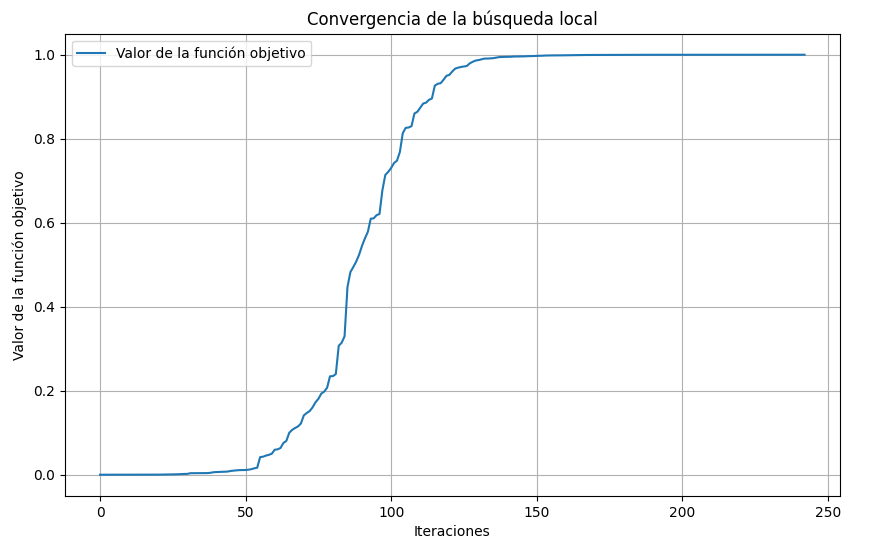
\includegraphics[width=\textwidth]{img/evolucion_dir_prohib_bl.png}
        \caption{Convergencia de búsqueda local para la señal de dirección prohibida}
        \label{fig:evol2}
\end{figure}




